\documentclass{anstrans}
%%%%%%%%%%%%%%%%%%%%%%%%%%%%%%%%%%%
\title{A DFEM Formulation of the Diffusion Equation on Arbitrary Polyhedral Grids}
\author{Michael W. Hackemack,$^{*}$ Jean C. Ragusa$^{*}$}

\institute{
$^{*}$Department of Nuclear Engineering, Texas A\&M Univeristy, 3133 TAMU, College Station, TX
}

\email{mike\_hack@tamu.edu \and jean.ragusa@tamu.edu}

% Optional disclaimer: remove this command to hide
%\disclaimer{Notice: This manuscript is a work of fiction. Any resemblance to actual articles, living or dead, is purely coincidental.}

%%%% packages and definitions (optional)
\usepackage{graphicx} % allows inclusion of graphics
\usepackage{booktabs} % nice rules (thick lines) for tables
\usepackage{microtype} % improves typography for PDF
%\usepackage{subfigure}
\usepackage{subcaption}
\usepackage{float}

\newcommand{\SN}{S$_N$}
\renewcommand{\vec}[1]{\bm{#1}} %vector is bold italic
\newcommand{\vd}{\bm{\cdot}} % slightly bold vector dot
\newcommand{\grad}{\vec{\nabla}} % gradient
\newcommand{\ud}{\mathop{}\!\mathrm{d}} % upright derivative symbol

\begin{document}
%%%%%%%%%%%%%%%%%%%%%%%%%%%%%%%%%%%%%%%%%%%%%%%%%%%%%%%%%%%%%%%%%%%%%%%%%%%%%%%%
\section{Introduction}

We present a Discontinuous Finite Element (DFEM) formulation of the radiation diffusion equation that is fully compatible with piece-wise linear basis functions on arbitrary polyhedral cells in 3D. The formulation is based on an Interior Penalty method that yields a symmetric positive definite matrix and can be used as a preconditioner for DFEM $S_N$ transport discretized using the same discontinuous basis functions. 

%%%%%%%%%%%%%%%%%%%%%%%%%%%%%%%%%%%%%%%%%%%%%%%%%%%%%%%%%%%%%%%%%%%%%%%%%%%%%%%%
\section{Theory}

The radiation diffusion equation is recalled:

\begin{equation} \label{eq:DIffEq}
- \vec{\nabla} \cdot D \vec{\nabla} \Phi(\vec{r}) + \sigma \Phi(\vec{r}) = q(\vec{r}), \qquad \vec{r} \in \mathcal{D}
\end{equation}

\noindent where $D$ is the diffusion coefficient, $\sigma$ is the absorption cross section, $q(\vec{r})$ is a source term that may consist of fission as well as some distributed source, and $\Phi(\vec{r})$ is the scalar flux solution. The boundary conditions are given by

\begin{equation} \label{eq:dirichlet_bndy}
\Phi \, =\Phi_0 \qquad \vec{r} \in \partial \mathcal{D}^d
\end{equation}

\noindent for the Dirichlet boundaries,

\begin{equation} \label{eq:neumann_bndy}
- D \partial_n \Phi \, = J_{0} \qquad \vec{r} \in \partial \mathcal{D}^n
\end{equation}

\noindent for the Neumann boundaries, and

\begin{equation} \label{eq:robin_bndy}
 \frac{1}{4} \Phi + \frac{1}{2} D \partial_n \Phi \, = J^{inc} \qquad \vec{r} \in \partial \mathcal{D}^r
\end{equation}

\noindent for the Robin boundaries where the whole domain boundary is $\partial \mathcal{D} \in \mathcal{D}^d \cup \mathcal{D}^n \cup \mathcal{D}^r$. $\partial_n = \vec{n} \cdot \vec{\nabla}$ is defined as the partial derivative along the outward normal to the surface.

%%%%%%%%%%%%%%%%%%%%%%%%%%%%%
\subsection{DFEM Formulation of the Diffusion Equation}
\label{sec::DFEM}
%%%%%%%%%%%%%%%%%%%%%%%%%%%%%

To solve Eq. (\ref{eq:DIffEq}) using discontinuous finite elements, we employ a symmetric interior penalty formulation for the diffusion equation \cite{ref::nitsche_IP,ref::arnold_1982_IP,riviere_book}. Interior penalty methods allow the use of discontinuous finite elements for this diffusion (elliptic) equation, whereby basis functions are defined on a given cell only and thus are discontinuous across cells. This results in the scalar flux solution also being discontinuous across cells. An advantage of such a discretization for the diffusion equation is that the same discontinuous finite element space can be employed for $S_N$ transport sweeps and Diffusion Synthetic Acceleration (DSA); see for instance, \cite{ref::DSA_2D_arb_poly,ref::DSA_wang_ragusa}. Several variants of the interior penalty for the diffusion equation have been developed; here we employed the symmetric variant that produces a linear system matrix that is symmetric positive definite \cite{riviere_book}. The symmetric interior penalty (SIP) weak form for the diffusion equation in Eq. (\ref{eq:DIffEq}) is given by:

\begin{equation}
a( \Phi, \Phi^*) = b(\Phi^*)
\label{eq:SIP_bilinear_form}
\end{equation}

\noindent with the following bilinear matrix:

\begin{equation}
\begin{aligned}
a( \Phi, \Phi^*) = \Big<  D \vec{\nabla}  \Phi , \vec{\nabla} \Phi^*  \Big>_{\mathcal{D}} + \Big<  \sigma   \Phi ,  \Phi^*  \Big>_{\mathcal{D}} \\
+  \frac{1}{2} \Big<    \Phi ,   \Phi^*\Big>_{\partial \mathcal{D}^r} +  \Big< \kappa_e^{SIP} [\![   \Phi ]\!] , [\![  \Phi^* ]\!]\Big>_{E_h^i}  \\ 
+ \Big<  [\![   \Phi ]\!] , \{\!\{  D \partial_n \Phi^* \}\!\}\Big>_{E_h^i} +\Big< \{\!\{  D \partial_n  \Phi \}\!\} , [\![  \Phi^* ]\!]\Big>_{E_h^i} \\
+ \Big< \kappa_e^{SIP}   \Phi ,   \Phi^* \Big>_{\partial \mathcal{D}^d} -\Big<   \Phi  ,  D \partial_n \Phi^* \Big>_{\partial \mathcal{D}^d} -\Big<   D \partial_n  \Phi ,   \Phi^*\Big>_{\partial \mathcal{D}^d}  
\end{aligned}
\label{eq::SIP_bilinear_op}
\end{equation}

\noindent and with the following linear form (i.e., right-hand-side):

\begin{equation}
\begin{aligned}
b(\Phi^*) = \Big<  q, \Phi^*  \Big>_{\mathcal{D}}  - \Big<   J_{0}, \Phi^*  \Big>_{\partial \mathcal{D}^n} +  2 \Big<   J_{inc}, \Phi^*  \Big>_{\partial \mathcal{D}^r} \\
 + \Big< \kappa_e^{SIP}   \Phi_0 ,   \Phi^* \Big>_{\partial \mathcal{D}^d} - \Big<   \Phi_0  ,  D \partial_n \Phi^* \Big>_{\partial \mathcal{D}^d}  \, .
\end{aligned}
\label{eq::SIP_rhs_op}
\end{equation}

The mean value and the jump of the scalar flux on the interior faces, $E_h^i$, are given by 

\begin{equation}
\{\!\{ \Phi \}\!\} = \frac{\Phi^{+} + \Phi^{-}}{2} \qquad \text{and} \qquad  [\![ \Phi ]\!] = \Phi^{+} - \Phi^{-},
\label{eq::mean_and_jump}
\end{equation}

\noindent respectively. The positive and negative orientations of the flux across the interface is defined by its trace:

\begin{equation}
\Phi^{\pm} \equiv \lim_{s \rightarrow 0^{\pm}} \Phi \left( \vec{r} + s \vec{n} \right),
\label{eq:trace}
\end{equation}

\noindent where the orientation of the face normal, $\vec{n}$, is irrelevant for interior faces and required to be oriented outwards for boundary faces (leaving only $\Phi^{-}$ for boundary nodes). This allows the direction of the interior normals to be arbitrarily selected for each interior face and the resulting orientation of across-face fluxes to be determined accordingly by Eq. (\ref{eq:trace}). Finally, the SIP penalty coefficient, $\kappa_e^{SIP}$, is given by

\begin{equation}
\kappa_e^{IP} \equiv 
\begin{cases}
\frac{c}{2} \left(  \frac{D^+}{h^+} + \frac{D^-}{h^-} \right) & e \in E_h^i\\ 
c \frac{D^-}{h^-}& e \in \partial \mathcal{D}
\end{cases},
\label{eq::SIP_penalty_term}
\end{equation}

\noindent where $h^{\pm}$ is the orthogonal projection of the face's area into the cell volumes and $c$ is a scaling constant (set to a value of 4 for this work as recommended by Kanschat \cite{kanschat2007discontinuous}).  From Eqs. (\ref{eq::SIP_bilinear_op}-\ref{eq::SIP_rhs_op}), one can see that the Dirichlet boundary conditions do not require direct adjustment of the system matrix as with continuous finite elements where they typically are strongly enforced. Also, the bilinear matrix is symmetric positive-definite and has been shown to be efficiently invertible with various preconditioning schemes using a Preconditioned Conjugate Gradient (PCG) solver \cite{ref::DSA_2D_arb_poly}.

%%%%%%%%%%%%%%%%%%%%%%%%%%%%%
\subsection{Basis Functions}
\label{sec::PWLD}
%%%%%%%%%%%%%%%%%%%%%%%%%%%%%
%
Since we are working on unstructured polyhedral meshes, we wish to utilize DFEM basis functions amenable to arbitrary geometric shapes. For $S_N$ transport sweeps, Adams and Stone derived a piece-wise linear discontinuous (PWLD) basis set for arbitrary polygons \cite{ref::PWLD_stone_adams_unstructured}, which was later extended to 3D shapes \cite{bailey2008phd}. In \cite{bailey_jcp_diffusion}, piece-wise linear {\it continuous} functions were used to solve the radiation diffusion equation on arbitrary polyhedra. Here, we extend this to {\it discontinuous} basis functions using SIP.
%
For a given arbitrary polyhedral cell, $K$, the PWLD basis function at vertex $j$ is given by
%
\begin{equation}
b_j(x,y,z) = t_j(x,y,z) + \sum_{f=1}^{F_j} \beta_{f,j} t_f(x,y,z) + \alpha_{K,j} t_c(x,y,z) .
\label{eq::3D_PWLD_basis_functions}
\end{equation}

\noindent $t_j$ is the standard linear function with unity at vertex $j$ that linearly decreases to zero to the cell center, the face center for each face that includes vertex $j$, and each vertex that shares an edge with vertex $j$. $t_c$ is the cell "tent" function which is unity at the cell center and linearly decreases to zero to each cell vertex and face center. $t_f$ is the face "tent" function which is unity at the face center and linearly decreases to zero at each vertex on that face and the cell center. $\alpha_{K,j}$ is the weight parameter for vertex $j$ in cell $K$, $\beta_{f,j}$ is the weight parameter for face $f$ touching cell vertex $j$, and $F_j$ is the number of faces touching vertex $j$. Like the previous work defining the PWLD method \cite{bailey2008phd}, we also choose to assume the cell and face weighting parameters are


\begin{equation}
\alpha_{K,j} = \frac{1}{N_K} \qquad \text{and} \qquad \beta_{f,j} = \frac{1}{N_f},
\label{eq::PWLD_weight_vals}
\end{equation}

\noindent respectively, where $N_K$ is the number of vertices in cell $K$ and $N_f$ is the number of vertices on face $f$, which leads to constant values of $\alpha$ and $\beta$ for each cell and face, respectively.

One can see from Eq. (\ref{eq::3D_PWLD_basis_functions}) that the contributions of the PWLD basis functions are generated by subtended tetrahedra along each face within a cell. As an example, a hexahedral cell would be comprised of 24 tetrahedral sub-cells.

%%%%%%%%%%%%%%%%%%%%%%%%%%%%%%%%%%%%%%%%%%%%%%%%%%%%%%%%%%%%%%%%%%%%%%%%%%%%%%%%
\section{Results and Analysis}

To show the efficacy of this DFEM formulation utilizing SIP with the PWLD basis functions, we will demonstrate that we can capture the linear interpolation of the FEM solution on different arbitrary polyhedral meshes. This will be shown by both capturing a purely linear solution as well as demonstrating the proper convergence rate of PWLD with the Method of Manufactured Solutions (MMS). We show results from three different 3D prismatic grids obtained by {\em extruding} in the axial dimension the 2D meshes shown in Figure \ref{fig::meshes}. These include a Cartesian mesh (Figure \ref{fig::cart_mesh}), an ordered triangular mesh (Figure \ref{fig::poly_mesh}), and a polygonal mesh (Figure \ref{fig::shes_mesh}). The polygonal 2D meshes were generated with the POLYMESHER MATLAB script \cite{talischi2012polymesher}, and the coarseness of the grids were achieved by limiting the maximum cell sizes. The varying refinement of the MMS problems will be carried out by both adding extrusion levels as well as refining the initial 2D meshes.



%%%%%%%%%%%%%%%%%%%%%%%%%%%%%
\subsection{Linear Solutions}
\label{sec::Linear}
%%%%%%%%%%%%%%%%%%%%%%%%%%%%%

To demonstrate the robustness of the PWLD basis functions on 3D polyhedra, we simulate a purely linear solution through a non-axial direction through the mesh. Robin boundary conditions are employed on opposite boundaries and homogeneous Neumann conditions are employed on all other boundaries and $\sigma = q = 0$. The midplane axial slice of the linear solution for each mesh is given in Figure \ref{fig::lin_sols} where, for visualization purposes, the mesh includes the subtended PWLD tetrahedra. One can see from the figures that the PWLD basis functions do indeed yield the proper smooth linear solution even on distorted spatial cells.


%%%%%%%%%%%%%%%%%%%%%%%%%%%%%
\subsection{MMS Solutions}
\label{sec::MMS}
%%%%%%%%%%%%%%%%%%%%%%%%%%%%%

As previously stated, the SIP formulation with the PWLD basis functions were also tested with MMS by both refining/coarsening the meshes in Figure \ref{fig::meshes} and adding axial extrusion levels. The refinement for the Cartesian and ordered triangular meshes was achieved by simply doubling the number of cell divisions in $x$ and $y$ and doubling the number of axial extrusions for each refinement level. The polygonal mesh was refined by reducing the maximum 2D polygon area by a factor of 4 and doubling the number of axial extrusions at each refinement level.

The exact solution tested was just a simple quadratic in 3D space given by Eq. (\ref{eq::mms_func}). The procedure varied the number of Degrees of Freedom for each mesh type from approximately $10^1$ to $ 10^5$. The error in the mesh refinement for each mesh type is presented in Figure \ref{fig::mms_err}. As expected, we acheived second-order spatial error reduction as seen in the $-2/3$ asymptotic slope. Indeed, the number of degrees of freedom is about proportional to the cell size, $N \propto 1/h^3$. Then, second-order spatial convergence is observed  when the error reduction behaves as the power $2/3$ in the number of degrees of freedom, i.e., $e \propto N^{-2/3}$. 

\begin{equation}
\Phi (x,y,z) = x \, (1-x) \, y \, (1-y) \, z \, (1-z)
\label{eq::mms_func}
\end{equation}



%%%%%%%%%%%%%%%%%%%%%%%%%%%%%%%%%%%%%%%%%%%%%%%%%%%%%%%%%%%%%%%%%%%%%%%%%%%%%%%%
\section{Conclusions}

We have presented a DFEM formulation of the diffusion equation using a modified form of an interior penalty method (SIP) with piece-wise linear discontinuous (PWLD) basis functions on arbitrary polyhedral meshes. Three mesh types were tested (Cartesian hexahedral cells, ordered triangular prisms, and arbitrary polygonal prisms) with the 3D grids formed by extrusion of 2D meshes. A purely linear solution is preserved with the PWLD basis functions even on distorted spatial cells and MMS demonstrates the proper second-order error reduction.


%%%%%%%%%%%%%%%%%%%%%%%%%%%%%%%%%%%%%%%%%%%%%%%%%%%%%%%%%%%%%%%%%%%%%%%%%%%%%%%%

\begin{figure}[]
\centering
\begin{subfigure}{.5\textwidth}
	\centering
	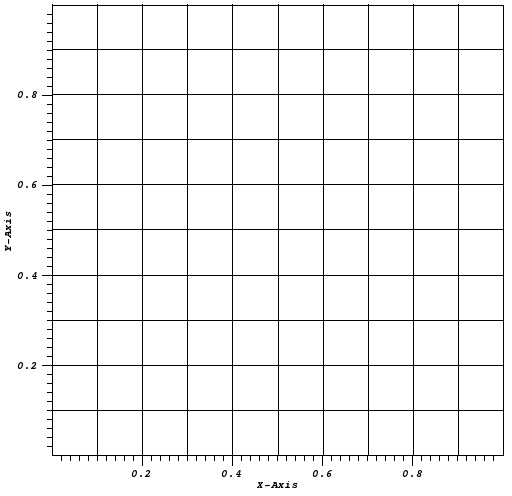
\includegraphics[scale=0.48]{cart_mesh.jpg}
	\caption{Cartesian Mesh}
	\label{fig::cart_mesh}
\end{subfigure}
\begin{subfigure}{.5\textwidth}
	\centering
	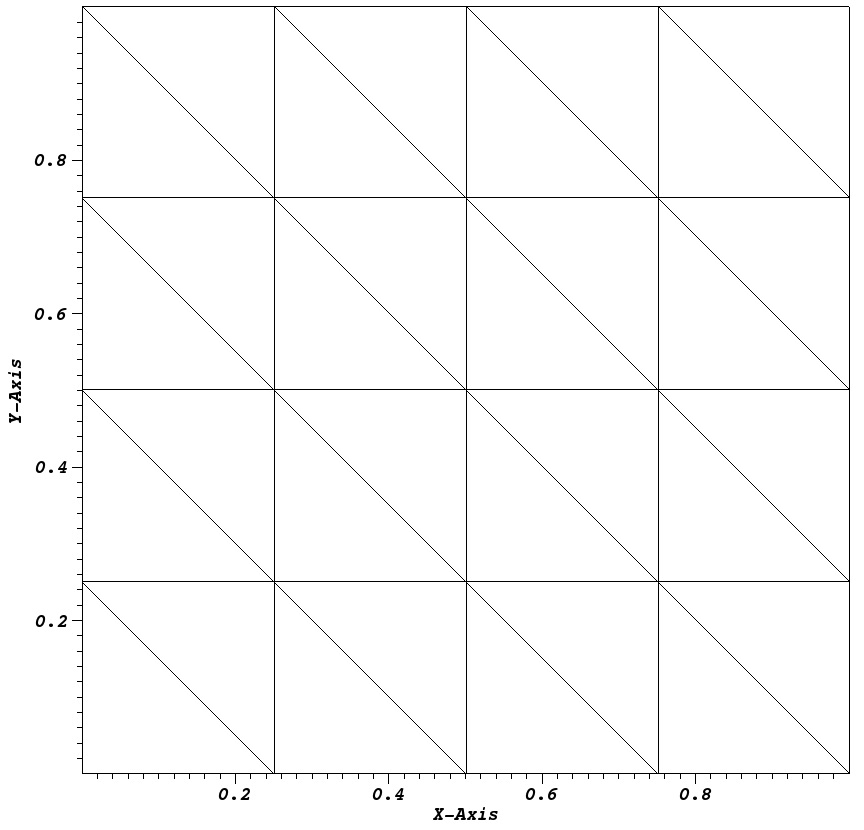
\includegraphics[scale=0.283]{visit0008.jpg}
	\caption{Ordered Triangular Mesh}
	\label{fig::poly_mesh}
\end{subfigure}
\begin{subfigure}{.5\textwidth}
	\centering
	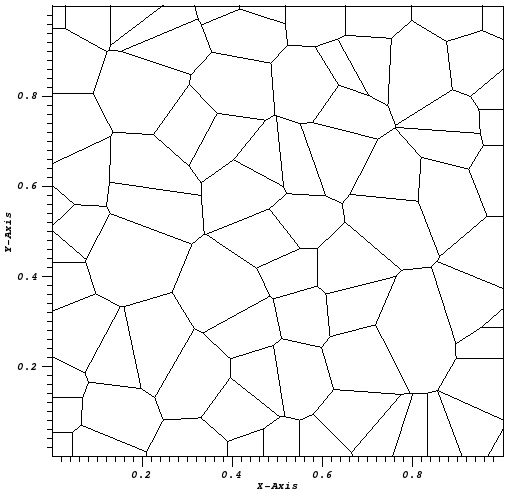
\includegraphics[scale=0.48]{poly_mesh.jpg}
	\caption{Polygonal Mesh}
	\label{fig::shes_mesh}
\end{subfigure}
\caption{The three 2D meshes extruded to form the 3D meshes.}
\label{fig::meshes}
\end{figure}


\begin{figure}[]
\centering
\begin{subfigure}{.5\textwidth}
	\centering
	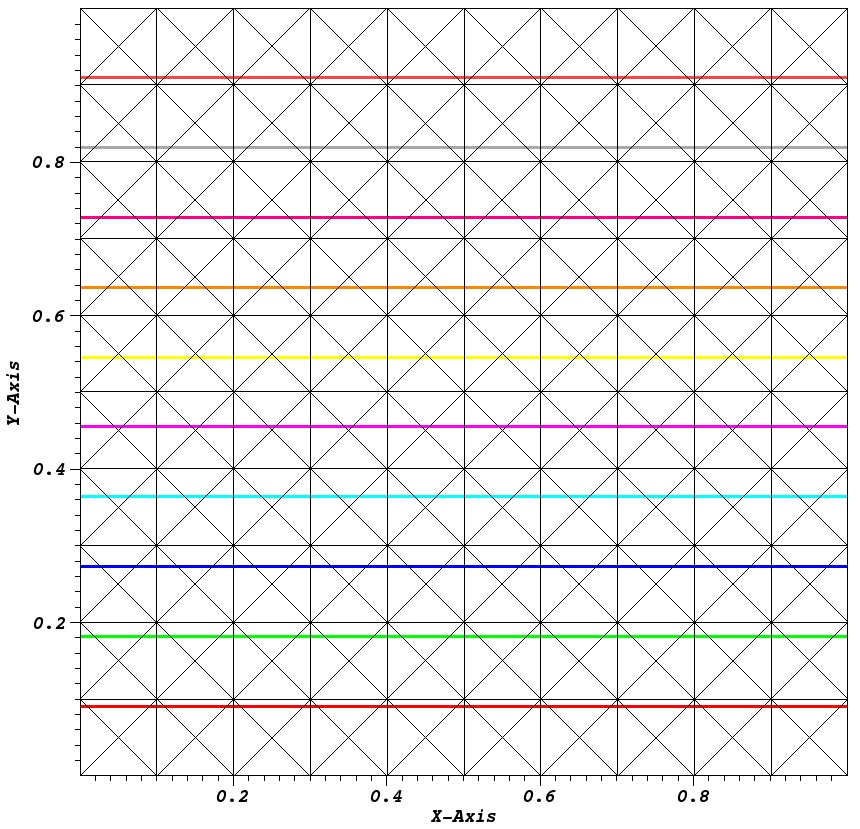
\includegraphics[scale=0.28]{visit0005.jpg}
	\caption{Cartesian Mesh}
	\label{fig::cart_lin_sol}
\end{subfigure}
\begin{subfigure}{.5\textwidth}
	\centering
	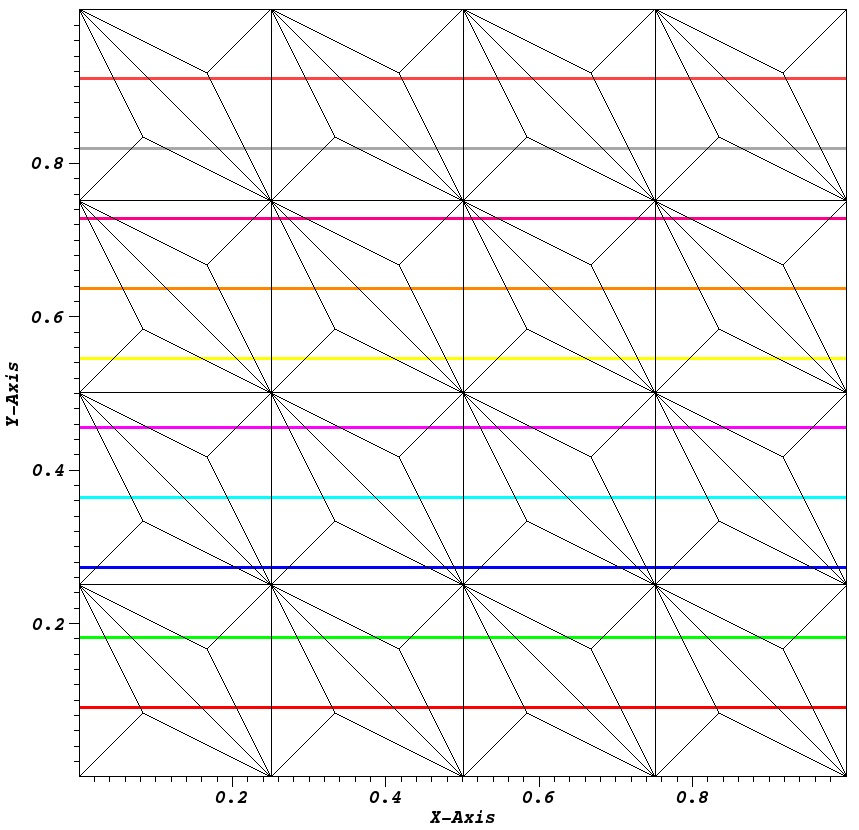
\includegraphics[scale=0.28]{visit0006.jpg}
	\caption{Ordered Triangular Mesh}
	\label{fig::poly_lin_sol}
\end{subfigure}
\begin{subfigure}{.5\textwidth}
	\centering
	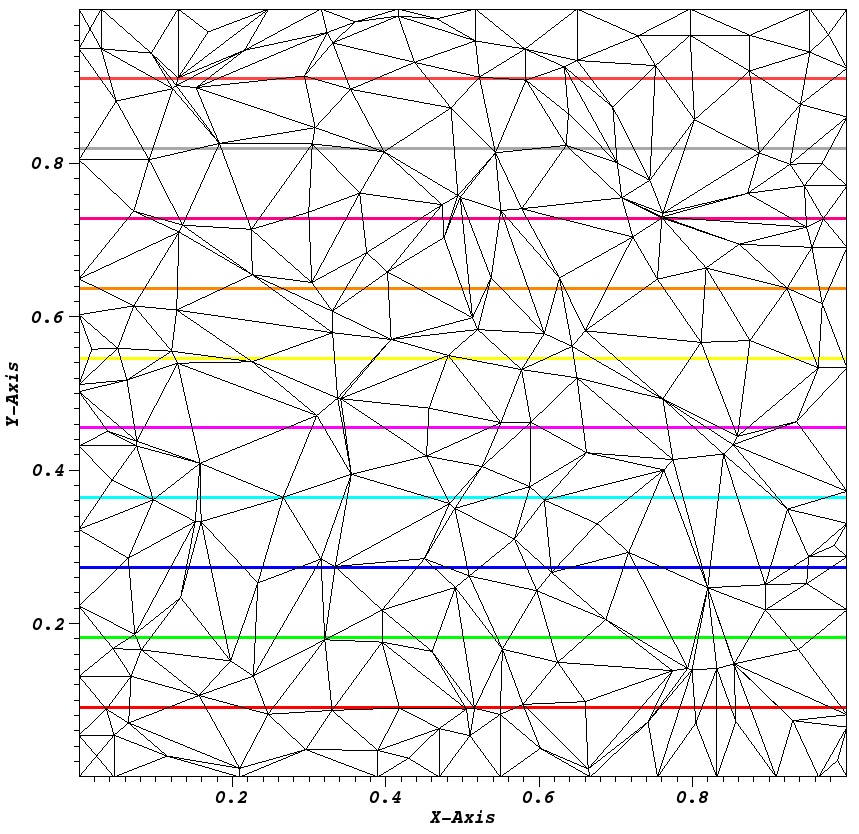
\includegraphics[scale=0.28]{visit0007.jpg}
	\caption{Polygonal Mesh}
	\label{fig::poly_lin_sol}
\end{subfigure}
\caption{An axial slice of the linear solution for the three meshes simulated.}
\label{fig::lin_sols}
\end{figure}

\begin{figure}[]
\centering
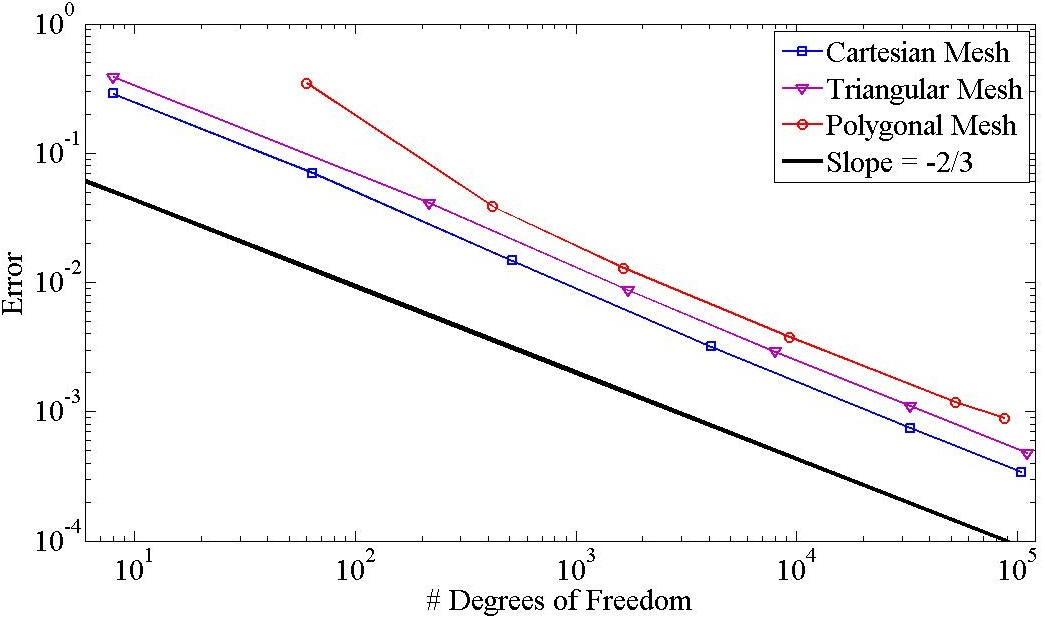
\includegraphics[scale=0.30]{mms_err.jpg}
\caption{MMS error convergence rate for the three mesh types.}
\label{fig::mms_err}
\end{figure}


%%%%%%%%%%%%%%%%%%%%%%%%%%%%%%%%%%%%%%%%%%%%%%%%%%%%%%%%%%%%%%%%%%%%%%%%%%%%%%%%
%\appendix
%\section{Appendix}

%%%%%%%%%%%%%%%%%%%%%%%%%%%%%%%%%%%%%%%%%%%%%%%%%%%%%%%%%%%%%%%%%%%%%%%%%%%%%%%%
%\section{Acknowledgments}
%This material is based upon work supported by the Department of Energy Rickover Fellowship Program in Nuclear Engineering.

%%%%%%%%%%%%%%%%%%%%%%%%%%%%%%%%%%%%%%%%%%%%%%%%%%%%%%%%%%%%%%%%%%%%%%%%%%%%%%%%
\bibliographystyle{ans}
\bibliography{references}

\end{document}

